\subsection{Introduction}
Maximum flow algorithms have historically been developed and analyzed within the context of network optimization, with early applications in logistics, transportation, and communication networks \cite{greig}. In the 1990s, maximum flow algorithms found application in computer vision.

In computer vision, many fundamental tasks such as image segmentation, stereo correspondence, and multi-view reconstruction can be modeled as energy minimization problems. These energy functions are often reducible to graph cut formulations, where finding a minimum cut corresponds to solving a maximum flow problem. Traditional algorithms like Edmonds-Karp or Push-Relabel algorithm offer theoretical guarantees but struggle with the large, grid-structured graphs typical of vision problems. 

Recognizing the specific structure of graphs instances for computer vision problems, Boykov and Kolmogorov proposed a max-flow algorithm optimized specifically for the structure and demands of vision applications. Their approach does not aim for the best worst-case complexity but instead achieves exceptional practical performance on the types of graphs encountered in computer vision.

\begin{figure}[h]
    \centering
    \begin{subfigure}[b]{0.3\textwidth}
        \centering
        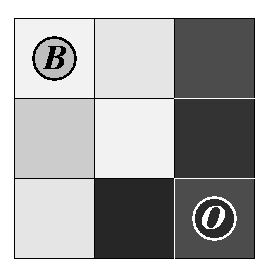
\includegraphics[width=\textwidth]{figures/iccv01-001.png}
        \caption{Image}
    \end{subfigure}
    \hfill
    \begin{subfigure}[b]{0.3\textwidth}
        \centering
        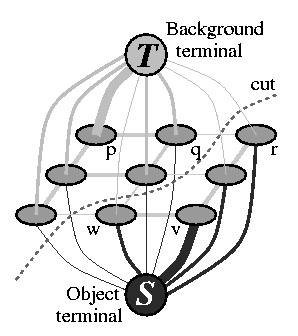
\includegraphics[width=\textwidth]{figures/iccv01-003.png}
        \caption{Corresponding Graph}
    \end{subfigure}
    \hfill
    \begin{subfigure}[b]{0.3\textwidth}
        \centering
        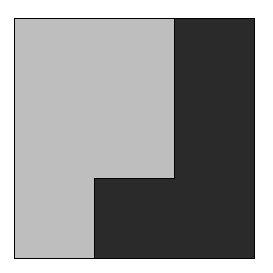
\includegraphics[width=\textwidth]{figures/iccv01-002.png}
        \caption{Result of segmentation}
    \end{subfigure}
    \caption{Example of a 2D segmentation for a 3x3 image. The edge weights in the corresponding graph align with pixel intensity. \cite{graphimage}
    }
\end{figure}

\subsection{Overview}

Boykov-Kolmogorov \cite{BK} algorithm belongs to the class of maximum flow algorithms based on finding augmenting paths.
In typical augmenting paths algorithms however the paths are searched using DFS or BFS and after each iteration a new search tree is built from scratch. Authors noticed that in computer vision problems this method is ineffective.

Instead of building new search tree for each augmenting path, the algorithm stores two search trees, one from the source and one from the sink. At each iteration one of the trees adopts a new node. An augmenting path is found once the trees "meet" each other. Once the path is saturated some nodes become disconnected from the search trees. A special procedure is implemented to either find a new path to the search trees or the nodes are removed from the trees.

\subsection{Definitions}

\begin{defn}
Search trees $S$ and
$T$ are trees with roots respectively at the source s and the sink t. 

In tree $S$ all edges from each parent
node to its children are non-saturated (have positive residual capacity), while in tree $T$ edges from children to their parents are non-saturated. A node cannot belong to both trees at the same time. The nodes that are not in $S$ or $T$ are called \emph{free}.
\end{defn}

\begin{defn}
A node $v$ is called \emph{active} if it is at the border of the search tree, ie it has a neighbour which does not belong to the same tree as $v$. 

A node that is not active is called \emph{passive}.
\end{defn}

\begin{defn}
We define $\text{tree\_capacity}(u,v)$ as:
\[
\text{tree\_capacity}(u,v) = 
\begin{cases}
c_f(u,v) & \text{if } u \in S, \\
c_f(v,u) & \text{if } u \in T,
\end{cases}
\]
where $c_f(u,v)$ denotes the residual capacity of edge $(u,v)$.
\end{defn}

\subsection{Algorithm}

As described previously, the algorithm maintains two search trees, $S$ and $T$, throughout its execution.  
They are represented using two arrays:
$$
\textsc{tree}[v] = 
\begin{cases}
S & \text{if } v \in S, \\
T & \text{if } v \in T, \\
\varnothing & \text{otherwise},
\end{cases}
$$
and
$$
\textsc{parent}[v] = 
\begin{cases} 
u \quad \text{if } u \text{ is the parent of } v \text{ in its respective search tree}, \\
\varnothing \text{ if } u \text{ is a free node or disconnected from its tree}. \\
\end{cases}
$$

The algorithm proceeds by repeatedly iterating a main loop until no augmenting path from the source to the sink exists. At that point, the maximum flow value has been determined and can be returned.
The main loop consists of three stages, growth, augmentation and adoption, explained in detail below the pseudocode.

\begin{algorithm}[H]
\caption{\textsc{Boykov-Kolmogorov  (Main Loop)}}
\begin{algorithmic}[1]
\State Initialize total flow $F \gets 0$
\State Initialize $S \gets \{s\}$, $T \gets \{t\}$
\State Initialize $A \gets \{s, t\}$ \Comment{Active nodes}
\State Initialize $O \gets \varnothing$ \Comment{Orphan nodes}
\While{\textbf{true}}
    \State $P \gets$ \Call{Grow}{}($A$)
    \If{$P = \varnothing$}
        \State \textbf{break}
    \EndIf
\State \text{augmented\_flow} $\gets$ \Call{Augment}{$P$}
\State $F \gets F +$ \text{augmented\_flow}
    \State \Call{AdoptOrphans}{}($O$)
\EndWhile
\State \Return{F}
\end{algorithmic}
\end{algorithm}

\paragraph*{1. Growth Stage.}  
In this stage, active nodes are selected, and their corresponding search trees expand toward neighboring nodes through edges with positive residual capacity. Newly added nodes are as active. The stage terminates either when the trees cannot grow anymore or when an augmenting path from the source $s$ to the sink $t$ is found.

An augmenting path is detected when a node in tree $S$ attempts to grow toward a node in tree $T$, or vice versa. The path is then reconstructed using the $\textsc{parent}[v]$ array.

\begin{algorithm}[H]
\caption{\textsc{Grow($A$)}}
\begin{algorithmic}[1]
\While{$A \neq \varnothing$}
    \State $v \gets$ $A$\text{.front}()
    \State $A$\text{.pop}()

    \State $\text{found\_path} \gets \text{false}$
    \ForAll{each $(v,w) \in E$}
        \If{\text{found\_path}}
            \State \textbf{break}
        \EndIf
        \If{$tree\_capacity(v, w) > 0$}
            \If{$\textsc{tree}[w] = \varnothing$}
                \State $\textsc{tree}[w] \gets \textsc{tree}[v]$
                \State $\textsc{parent}[w] \gets v$
                \State \text{active.push}{$(w)$}
            \ElsIf{$\textsc{tree}[w] \neq \textsc{tree}[v]$}
                \If{$\textsc{tree}[v] = \texttt{SOURCE}$}
                    \State $\text{spath} \gets v$, $\text{tpath} \gets w$ \Comment{Store the found path}
                \Else
                    \State $\text{spath} \gets w$, $\text{tpath} \gets v$
                \EndIf
                \State $\text{found\_path} \gets \text{true}$
                \State \text{active.push}{$(w)$}
                \State \textbf{break}
            \EndIf
        \EndIf
    \EndFor
    \If{\text{found\_path}}
        \State \Return $\text{true}$
    \EndIf
\EndWhile
\State \Return $\text{false}$
\end{algorithmic}
\end{algorithm}

\paragraph*{2. Augmentation Stage.}  
Once an augmenting path is found, the algorithm computes the bottleneck capacity $\Delta$ along the path and pushes flow of value $\Delta$ through the network.

For every edge $(p, q)$ on the augmenting path that becomes saturated, the algorithm performs the following:
\begin{itemize}
    \item If both $p$ and $q$ belong to tree $S$, then $q$ is disconnected from the search tree (i.e., $\textsc{parent}[q] \gets \varnothing$) and added to the set of orphans $O$.
    \item If both $p$ and $q$ belong to tree $T$, then $p$ is disconnected from the search tree and added to $O$.
\end{itemize}

This process may break the trees into disconnected forests, which are restored in the next stage.

\begin{algorithm}[H]
\caption{\textsc{Augment}($P$)} 
\begin{algorithmic}[1]
\State $\Delta \gets \min_{e \in P}\{c_f(e) \}$ \Comment{Find the bottleneck capacity $\Delta$ on path $P$}
\For{each edge $e \in P$}
    \State \textsc{Push}($e,\Delta$) \Comment{Push flow $\Delta$ through all edges in $P$}
\EndFor
\For{each edge $(u,v) \in P$}
    \If{$tree\_capacity(u,v) = 0$}
        \If{$\textsc{tree}[u] = \textsc{tree}[v] = S$}
            \State $\textsc{parent}[v] \gets \varnothing$
            \State $O \gets O \cup \{v\}$ \Comment{mark $q$ as orphan}
        \ElsIf{$\textsc{tree}[u] = \textsc{tree}[v] = T$}
            \State $\textsc{parent}[u] \gets \varnothing$
            \State $O \gets O \cup \{u\}$ \Comment{mark $u$ as orphan}
        \EndIf
    \EndIf
\EndFor
\State \Return $\Delta$
\end{algorithmic}
\end{algorithm}

\paragraph*{3. Adoption Stage.}  
In the adoption stage, the algorithm attempts to reattach orphaned nodes to their respective trees. For each orphan node, a new parent is looked for among its neighbors. A node $q$ is a valid new parent of an orphan $p$ if:
\begin{itemize}
    \item $q$ belongs to the same tree as $p$,
    \item the residual capacity $\textit{tree\_capacity}(q, p)$ is positive,
    \item the path from $q$ to the root of the tree is valid (i.e., all nodes along the path have defined parents).
\end{itemize}

If such a node $q$ is found, the orphan is reattached to the tree by setting $\textsc{parent}[p] \gets q$. If no such parent can be found, $p$ becomes a free node, and any of its children in the tree are also added to the orphan set. This stage continues until all orphans have been processed.

\begin{algorithm}[H]
\caption{\textsc{Adopt}($O$)}
\begin{algorithmic}[1]
\While{$O$ is not empty}
    \State $u \gets$ $O$\text{.front}()
    \State $found\_new\_parent \gets \text{false}$
    \For{ each edge $(u,v) \in E$}
        \If{$\textsc{tree}[v] = \textsc{tree}[u]$ \textbf{and} $tree\_capacity(u,v) > 0$ \textbf{and} $v$ has a valid path to root}
            \State $\textsc{parent}[u] \gets v$
            \State $found\_new\_parent \gets \text{true}$
            \State \textbf{break}
        \EndIf
    \EndFor
    \If{\textbf{not} $found\_new\_parent$}
        \For{each neighbor $v$ of $u$}
            \If{$\textsc{tree}[v] = \textsc{tree}[u]$}
                \If{$tree\_capacity(u,v) > 0$}
                    \State \text{active.push}($v$)
                \EndIf
                \If{$\textsc{parent}[v] = u$}
                    \State $\textsc{parent}[v] \gets \varnothing$
                    \State $O$\text{.push}($v$)
                \EndIf
            \EndIf
        \EndFor
        \State $\textsc{tree}[u] \gets \varnothing$
    \EndIf
\EndWhile
\end{algorithmic}
\end{algorithm}

\subsection{Correctness and Complexity}

We aim to establish two main properties of the algorithm: its termination and its computational complexity.

\paragraph*{Correctness.}  
To prove correctness, we must show that the algorithm terminates and produces a valid maximum flow.

\begin{itemize}
    \item \textbf{Termination:}  
    Clearly the main loop will be executed a finite number of times since each iteration finds an augmenting path with bottleneck capacity of at least 1.
The growth and augment stage are linear in terms of network size and therefore terminate as well.
The fact that the adoption stage is finite follows from the following lemma:
\begin{lemma}
Each node can become an orphan at most once in a single stage.
\end{lemma}
\begin{proof}
Consider a processed orphan $u$. If $u$ becomes a free node then by definition it will no longer take part in the adoption stage. Then assume that $u$ receives a new parent $v$. The node $v$ must satisfy the condition that all nodes along the path from $v$ to the root have defined parents. Since a node can become an orphan in the adoption stage only if its ancestor becomes one and all ancestors of $u$ have defined parents, then it is clear that $u$ cannot become an orphan again.
\end{proof}

    \item \textbf{Maximum Flow:}
    The algorithm terminates when there is no edges with positive residual capacities from nodes belonging to search trees. Then the trees are disconnected in the residual graph and therefore the flow is maximal.
    
\end{itemize}

\paragraph*{Complexity.}  
Unlike in algorithms such as Dinic’s or the Malhotra-Kumar-Maheshwari (MKM) algorithm, the augmenting paths found by the Boykov-Kolmogorov algorithm are not necessarily shortest paths. Thus, the bounds established for those algorithms do not directly apply here.

The only general upper bound we can establish is the trivial one:
$$O(|V|^2|E||f|)$$
where $|f|$ is the value of the maximum flow. This follows from the fact that each augmentation increases the total flow by at least one (provided the capacites are integers), and each operation within a stage is polynomial with respect to the graph size.
